\documentclass[tikz,border=5pt]{standalone}
\usepackage[utf8]{inputenc}
\usepackage[T1]{fontenc}
\usepackage{amsmath,amssymb}
\usepackage{lmodern}
\usetikzlibrary{arrows.meta,calc}

\definecolor{ink}{HTML}{1d1d1f}
\definecolor{sub}{HTML}{515154}
\definecolor{muted}{HTML}{6e6e73}
\definecolor{border}{HTML}{d2d2d7}
\definecolor{mist}{HTML}{f5f5f7}
\definecolor{amber}{HTML}{c76008}
\definecolor{amberbright}{HTML}{ff9f0a}
\definecolor{amberfill}{HTML}{fff3e0}
\definecolor{blue}{HTML}{0066cc}
\definecolor{bluebright}{HTML}{2997ff}
\definecolor{red}{HTML}{d70015}
\definecolor{redbright}{HTML}{ff453a}
\definecolor{redbeam}{HTML}{ffe4df}

\begin{document}
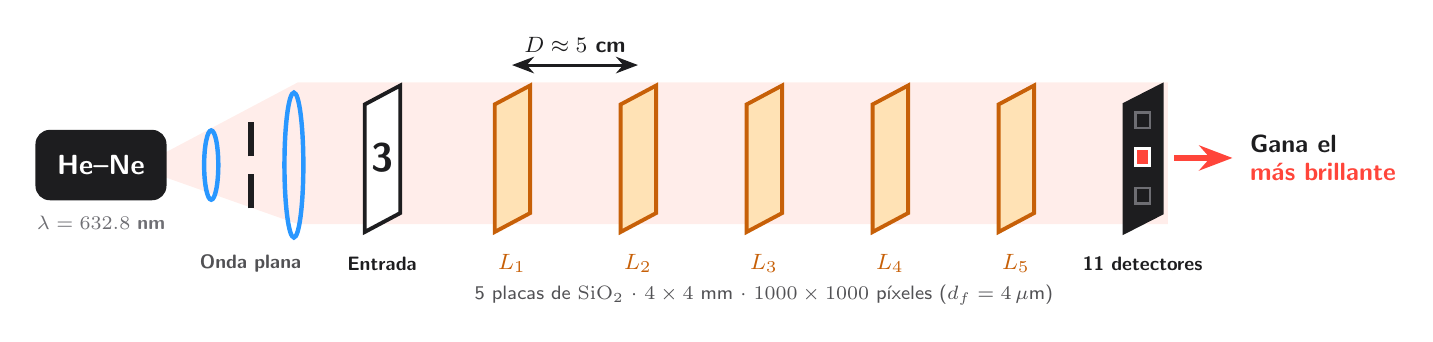
\begin{tikzpicture}[font=\sffamily,>=Stealth]

% Haz rojo expandido (fondo)
\fill[redbeam,opacity=0.65] (1.65,1.82) -- (3.35,2.72) -- (14.40,2.72) -- (14.40,0.92) -- (3.35,0.92) -- (1.65,1.52) -- cycle;

% Fuente He-Ne
\node[draw=ink,fill=ink,rounded corners=5pt,minimum width=1.65cm,minimum height=0.88cm,text=white,font=\sffamily\bfseries\normalsize] (hene) at (0.85,1.67) {He--Ne};
\node[font=\sffamily\scriptsize\bfseries,text=muted] at (0.85,0.94) {$\lambda = 632.8\text{ nm}$};

% Óptica de colimación (lente + pinhole + lente)
\draw[bluebright,line width=1.6pt] (2.25,1.67) ellipse (0.09cm and 0.44cm);
\draw[ink,line width=2.2pt] (2.75,1.12) -- (2.75,1.56);
\draw[ink,line width=2.2pt] (2.75,1.78) -- (2.75,2.22);
\draw[bluebright,line width=1.6pt] (3.30,1.67) ellipse (0.12cm and 0.92cm);
\node[font=\sffamily\scriptsize\bfseries,text=sub] at (2.75,0.42) {Onda plana};

% Entrada (máscara de Cr con dígito 3)
\draw[draw=ink,fill=white,line width=1.4pt] (4.20,0.82) -- (4.65,1.06) -- (4.65,2.68) -- (4.20,2.44) -- cycle;
\node[font=\sffamily\bfseries\Large,text=ink] at (4.42,1.76) {3};
\node[font=\sffamily\scriptsize\bfseries,text=ink] at (4.42,0.42) {Entrada};

% 5 Placas difractivas de sílice fundida
\foreach \i/\x in {1/5.85, 2/7.45, 3/9.05, 4/10.65, 5/12.25} {
  \draw[draw=amber,fill=amberbright!30,line width=1.4pt]
    (\x,0.82) -- (\x+0.45,1.06) -- (\x+0.45,2.68) -- (\x,2.44) -- cycle;
  \node[font=\sffamily\footnotesize\bfseries,text=amber] at (\x+0.22,0.42) {$L_{\i}$};
}

% Cota de separación D entre L1 y L2
\draw[<->,ink,line width=1.1pt] (6.07,2.94) -- (7.67,2.94);
\node[above,font=\sffamily\footnotesize\bfseries,text=ink] at (6.87,2.98) {$D \approx 5\text{ cm}$};

% Nota descriptiva inferior
\node[font=\sffamily\scriptsize,text=sub] at (9.27,0.02)
  {5 placas de $\mathrm{SiO_2}$ $\cdot$ $4\times 4\text{ mm}$ $\cdot$ $1000\times 1000$ píxeles ($d_f = 4\,\mu\text{m}$)};

% Plano de 11 detectores
\draw[draw=ink,fill=ink,line width=1.4pt] (13.85,0.82) -- (14.32,1.06) -- (14.32,2.68) -- (13.85,2.44) -- cycle;
\draw[muted,line width=0.9pt] (13.99,2.14) rectangle (14.17,2.34);
\draw[white,fill=redbright,line width=1.0pt] (13.99,1.66) rectangle (14.17,1.88);
\draw[muted,line width=0.9pt] (13.99,1.18) rectangle (14.17,1.38);
\node[font=\sffamily\scriptsize\bfseries,text=ink] at (14.08,0.42) {11 detectores};

% Salida / decisión
\draw[->,redbright,line width=2.0pt] (14.48,1.76) -- (15.22,1.76);
\node[anchor=west,font=\sffamily\small\bfseries,text=ink,align=left] at (15.32,1.76)
  {Gana el\\[-1pt]\color{redbright}más brillante};

\end{tikzpicture}
\end{document}
